% !TEX TS-program = XeLaTeX+MakeIndex+BibTeX
% !TEX encoding = UTF-8 Unicode

\documentclass[12pt]{article}

\usepackage[utf8]{inputenc}
\usepackage[brazilian]{babel}

\usepackage{fontspec}
\setmainfont{Linux Libertine O}
\linespread{1.05}

%%% PAGE DIMENSIONS
\usepackage{geometry} % to change the page dimensions
\geometry{a4paper}    % or letterpaper (US) or a5paper or...

% \geometry{margin=2in} % for example, change the margins to 2 inches all round
% \geometry{landscape}  % set up the page for landscape

\usepackage{graphicx} % support the \includegraphics command and options

% \usepackage[parfill]{parskip} % Activate to begin paragraphs with an empty line rather than an indent

%%% PACKAGES

\usepackage{amsfonts}
\usepackage{color}
\usepackage[colorinlistoftodos]{todonotes}
%\usepackage{booktabs} % for much better looking tables
%\usepackage{array}    % for better arrays (eg matrices) in maths
%\usepackage{paralist} % very flexible & customisable lists (eg. enumerate/itemize, etc.)
\usepackage{verbatim}  % adds environment for commenting out blocks of text & for better verbatim
\usepackage{microtype}
\usepackage[numbers]{natbib}
%\usepackage{subfig} % make it possible to include more than one captioned figure/table in a single float
% These packages are all incorporated in the memoir class to one degree or another...
\usepackage[hidelinks]{hyperref}

\usepackage{listings}


% For Computer Modern:
%\def\Cpp{{C\nolinebreak[4]\hspace{-.05em}\raisebox{.4ex}{\tiny\bf ++}}}
% For Linux Libertine G
\def\Cpp{{C\nolinebreak[4]\raisebox{.20ex}{\small\bf++}}}

%\newcommand{\todo}[1]{\textsf{\color{red}#1}}

%%% END Article customizations

\title{Irrigação e monitoramento de horta escolar\\ como tema de iniciação à computação na educação básica}
% ou 'iniciação à programação'

%Acredito que tenha que trocar o título para algo que represente melhor o trabalho

\author{Lucas Ferreira da Silva \\ \emph{Universidade Federal de Santa Maria}}
%\date{} % Activate to display a given date or no date (if empty), otherwise the current date is printed 

\begin{document}
	\maketitle
	
	\section{Identificação}
	
	\begin{description} \itemsep 0pt
		\item[Resumo:] ~\\
 Nos tempos atuais, com os constantes avanços tecnológicos, cada vez fica mais evidente a necessidade e a importância de se saber programar. Escolas são levadas a iniciar digitalmente seus alunos desde cedo, porém, muitas vezes, essa introdução fica apenas no âmbito de ensinar como as crianças e jovens podem usufruir dos recursos tecnológicos, não os incentivando a serem os modificadores ou até mesmo os criadores de tais recursos. Este cenário é decorrente, na maioria das vezes, da dificuldade de se abordar os conteúdos relacionados a programação dentro da sala de aula, pois ela ainda é vista como algo muito complexo até mesmo pelos professores e, para contornar esse problema, são necessárias estratégias didáticas mais eficientes e dinâmicas. Pensando nisso, no presente trabalho, pretende-se explorar o desenvolvimento de um sistema de irrigação e monitoramento de uma horta escolar como tema para o ensino de programação em escolas de educação básica, com o intuito de unir a teoria e a prática em uma atividade que possibilite uma maior dinamicidade no processo de ensino. Para a concretização da iniciativa, será realizada uma busca e seleção sistemáticas dos elementos necessários para se trabalhar com crianças e jovens, desde recursos de hardware para que o projeto de automação seja viável enquanto estratégia didática, como também ferramentas de software que possibilitem que os alunos programem os componentes do sistema em questão. Estes recursos serão organizados e apresentados em diversos formatos e meios, visando seu reaproveitamento em diferentes tempos e espaços.
	
		 
		\item[Período de execução:] agosto de 2018 a dezembro de 2018
		\item[Unidades participantes:] ~\\ Curso de Ciência da Computação e Departamento de Linguagens e Sistemas de Computação
        
		\item[Área de conhecimento:] Ciência da Computação
		\item[Linha de Pesquisa:] Sistemas Paralelos e Distribuídos
		\item[Participantes:] ~\\ Profª Andrea Schwertner Charão -- Orientadora \\ Lucas Ferreira da Silva -- Orientando
	\end{description}
	
	\section{Introdução}
	A tecnologia vem revolucionando a humanidade: a cada dia passa, uma nova solução digital surge para facilitar a vida das pessoas. Inovações tecnológicas, para os mais variados fins, surgem a todo momento, seja como um novo aplicativo para o smartphone ou até mesmo na forma de alguma ferramenta para solução de algum problema cotidiano. 
    
    Todavia, para um indivíduo acompanhar essa evolução de velocidade exponencial, já não basta mais ser apenas um bom usuário, é necessário compreender como essa realidade funciona e saber manuseá-la a fim de obter o melhor que ela tem a oferecer. Desta forma, saber programação tem se tornado indispensável, pois é a partir dela que passa a ser possível moldar os recursos digitais a favor dos seus usuários.

Neste contexto, há um crescente incentivo para que escolas não se atenham apenas na introdução dos seus alunos ao meio digital, mas sim os preparem para serem parte dos construtores dessa realidade. Para isso, é necessário que o pensamento computacional seja incorporado ao currículo das escolas e os preceitos da lógica de programação sejam apresentados desde cedo, fazendo com que esse conhecimento seja construído junto ao desenvolvimento escolar do aluno, pois, como é reforçado por \cite{Martinez:2015:CPE:2729094.2742599}, mesmo alunos de faixas etárias mais baixas (5 e 6 anos de idade) são capazes de aprender os fundamentos básicos da lógica computacional e aplicá-la em algum contexto.

	No entanto, um dos maiores desafios ao se trabalhar com crianças e jovens é acerca da didática utilizada para ensinar os conceitos relacionados a programação, já que esse tema ainda é visto como algo bastante complexo até mesmo para os professores, cuja experiência na abordagem desse tema, é fator influenciador, seja de forma positiva ou até mesmo negativa, no processo de aprendizagem do aluno, reafirma \cite{Fagin:2003:MER:611892.611994}. Para contornar esse obstáculo, é importante que se adotem didáticas mais dinâmicas, que se aproximem do dia a dia dos alunos, mostrando a aplicabilidade e a utilidade do que lhes está sendo ensinado.
	
    Dentre as várias metodologias de ensino de programação, ultimamente uma abordagem que vem ganhando bastante força é a do movimento "maker", em que os alunos são instigados a “pôr a mão na massa” durante o processo de aprendizagem, objetivando a criação de um ambiente educacional mais colaborativo e que explore a criatividade e a autonomia das crianças e jovens. Segundo \cite{digitalFab}, as possibilidades desse método estão associadas com teorias pedagógicas de Seymour Papert e Paulo Freire, em que a escola se torna mais conectada com a realidade do jovem e com os problemas que ele enfrenta no cotidiano, o que contribui para o seu aprendizado.
    
    O movimento maker, conforme \cite{estadao}, tem sido visto como uma das mais promissoras alternativas para a mudança do sistema educacional atual, já que suas características o tornam de fácil integração com várias disciplinas e influencia significativamente na compreensão dos mais variados conteúdos, pois faz com que o aluno interaja e busque o entendimento mais profundo de como e o porquê da necessidade de se aprender determinada matéria.
    
    Desta forma, recursos como a plataforma Arduino, Lego, impressoras 3D, entre outros, passaram a ser grandes aliados na concretização da educação "maker", pois possibilitam a criação, prototipação, montagem, programação e reprogramação dos diversos projetos desenvolvidos pelos alunos que, com esses recursos palpáveis, podem transformar sua imaginação em algo físico, além de contribuir para que os mesmos identifiquem problemas relevantes ao meio  ao qual estão inseridos e busquem soluções colaborativas para essas necessidades.


	\section{Objetivos}
A seguir são explicados os objetivos gerais e específicos do presente trabalho.
	\subsection{Objetivo Geral}
	O presente trabalho possui como principal objetivo apresentar uma proposta de ensino de programação para alunos do ensino médio, utilizando ferramentas de aprendizado de programação e/ou robótica para tornar tal tarefa mais dinâmica e atrativa para os alunos. O contexto das atividades a serem realizadas será o projeto da automatização da irrigação e monitoramento de uma horta escolar.   
    
	\subsection{Objetivos Específicos}
	
	\begin{itemize}
    	\item Realizar uma busca aprofundada referente as alternativas de hardware necessárias para a implementação do sistema de irrigação e monitoramento da horta escolar, levando em consideração aspectos como custo, disponibilidade, eficiência e quantidade de recursos;
    
		\item Investigar ferramentas que abstraiam a complexidade da programação dos sensores e atuadores do projeto, visando viabilizar o sistema de automação em questão para ser utilizado também para fins didáticos;
        
        \item  Explorar o cenário de uma horta escolar enquanto ambiente passível de automação, tanto no que tange a coleta de dados que podem ser utilizados posteriormente, quanto no âmbito de automatização de atividades de manejo, como a irrigação.  
		
        \item Obter um sistema que possibilite o monitoramento e coleta de alguns dados da horta em questão, possibilitando assim, criar uma base de dados que permita inferir informações importantes do ambiente e sua influência nas plantas, bem como propiciar o uso de tais informações no âmbito escolar de forma multidisciplinar;
        
		\item Instigar os alunos a propor melhorias para o projeto de irrigação e monitoramento da horta escolar a partir dos dados que vão sendo coletados pelas soluções que os próprios alunos vão desenvolvendo no decorrer das atividades.
	\end{itemize}
	
	\section{Justificativa}	
Com a tecnologia evoluindo em uma velocidade nunca antes vista, atualmente saber programação já é quase que indispensável para acompanhar e usufruir das novas facilidades que surgem diariamente. Assim, os conceitos relativos à lógica computacional estão sendo introduzidos para as crianças e jovens cada vez mais cedo, principalmente em países desenvolvidos. Porém, a programação muitas vezes pode ser vista como um conteúdo demasiadamente complexo, de modo que professores enfrentam o desafio de escolher a abordagem a ser adotada para que os alunos não vejam a programação como algo complicado,  descontextualizado e, por sua vez, maçante. Uma abordagem que promova o aprendizado significativo é desejável e  pode fazer toda diferença no processo de aprendizagem das crianças e dos jovens.

Neste contexto, uma das alternativas baseia-se na transmissão dos preceitos de programação de uma forma lúdica e ao mesmo tempo palpável, em que recursos como placas de prototipagem, como a plataforma Arduino e ESPduino, são os instrumentos principais para aliar a teoria com a prática. Isso possibilita que se explore não somente conhecimentos relacionados à programação, mas também à integração desses com o ambiente no qual a escola e o aluno estão inseridos. Além disso, conforme \cite{Litts:2017:UHS:3017680.3017740}, trabalhar com esses recursos pode ser inicialmente um tanto desafiador para os alunos, porém, com uma abordagem de ensino colaborativa onde todos constroem o conhecimento e aprendem juntos, é mais fácil de sanar as possíveis diferenças de aprendizado que podem surgir entre os alunos e, por consequência, a turma progride junto.

Um desses ambientes é a horta escolar, que possui um grande potencial interdisciplinar que, muitas vezes, não é suficientemente explorado e acaba sendo esquecido. Desta forma, aliar os recursos de sensores e atuadores das plataformas Arduino e ESPduino, com o ensino de programação, ambos aplicados no contexto de uma horta escolar, pode revelar uma estratégia didática que promove a interdisciplinaridade, coletividade e criatividade de uma forma dinâmica e aplicada no cotidiano do aluno. 
	
	\section{Revisão da Literatura}
	Nesta seção são apresentados alguns conceitos e ferramentas citados no decorrer do presente projeto, cuja a compreensão contribui para a assimilação do assunto abordado neste trabalho.
    
	\subsection{Programação visual através de blocos}
	A programação visual pode ser vista como uma forma de abstração da parte léxica e/ou sintática dos comandos de uma linguagem de programação convencional, transformando as complexas sentenças em recursos visuais que consigam expressar a mesma lógica da linguagem só que de uma forma mais clara. Dentre os recursos visuais geralmente utilizados nesse tipo de abordagem estão os blocos de encaixe, que transformam cada parte do código em um bloco que pode ser ligado a outros, possibilitando assim que a lógica do algoritmo possa ser construída como se fosse um quebra-cabeças.
    
\begin{figure}[!ht]
\centering
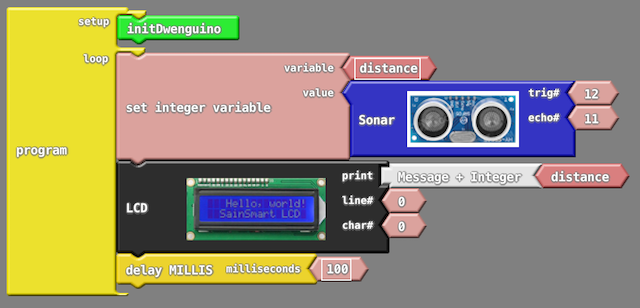
\includegraphics[keepaspectratio, width=0.8
\textwidth]{images/ardublock.png}
\caption{Estrutura de programa utilizando a plataforma Ardublock}
\label{fig:arduino}
\end{figure}

    Neste projeto, o recurso de programação visual proposto é o de programação através de blocos, utilizando a plataforma Ardublock \cite{ardublock}, uma aplicação desenvolvida por meio da linguagem Java e que objetiva abstrair de forma visual os códigos da linguagem de programação utilizada por placas de prototipagem como Arduino e ESPduino.
  
    O Ardublock pode ser facilmente instalado na IDE do Arduino, sendo necessário apenas o download dos arquivos (disponíveis no site do desenvolvedor) e posteriormente incorporar na IDE como uma nova ferramenta. Sua utilização é bastante simples, muito semelhante a outros recursos mais populares como por exemplo o Blockly, além de possuir abstração para quase a totalidade das funções da linguagem utilizada pelo Arduino e seus similares. 
    
	\subsection{Plataformas de prototipagem no ensino de programação}
    As plataformas de prototipagem de hardware surgem como ferramentas facilitadoras para o projeto, prototipagem e aprendizado dos preceitos de eletrônica e microcontroladores, de uma forma mais fácil e de menor custo, pois permitem que, com uma mesma plataforma de prototipagem, sejam realizados vários projetos distintos e de maneira bastante simples.
    
    Dada as facilidades propiciadas por essas plataformas para a confecção e aprendizado de novos projetos de hardware, elas acabaram se popularizando como alternativas para o ensino de conceitos básicos tanto de eletrônica quanto de programação. Para o ensino de programação, a maior contribuição desses recursos está na dinamicidade que proporcionam, pois possibilitam que o aluno possa manusear, montar, programar e reprogramar tais artefatos, tornando visível e palpável a lógica empregada pelo aluno, fazendo com que o mesmo assimile de forma mais efetiva os conceitos em questão. 
    
    No presente projeto, as plataformas Arduino e ESPduino foram selecionadas como as alternativas a serem utilizadas como os recursos auxiliadores no ensino de programação.    
    
    \subsubsection{Arduino}
Arduino é uma plataforma para prototipagem e projeto de eletrônica e hardware em geral. Criada em 2005, por um grupo de pesquisadores formado por: Massimo Banzi, David Cuartielles, Tom Igoe, Gianluca Martino e David Mellis, a plataforma segue o conceito de hardware e software livre, possibilitando que qualquer pessoa possa montar, modificar e personalizar a plataforma, partindo da especificação de hardware base do projeto \cite{arduino}.

\begin{figure}[!ht]
\centering
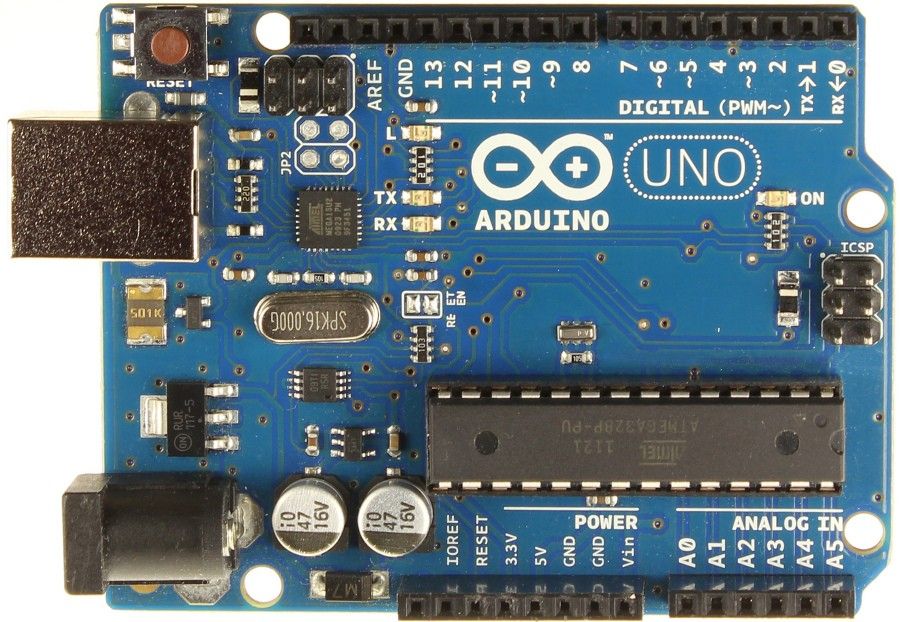
\includegraphics[keepaspectratio, width=0.4
\textwidth]{images/arduino_uno.jpg}
\caption{Arduino UNO R3}
\label{fig:arduino}
\end{figure}

A placa é composta por um microcontrolador Atmel AVR com suporte para entrada e saída, e pode ser conectada a um computador via USB e reprogramada por meio de uma linguagem de programação baseada em C/C++. Após programado o microcontrolador pode ser utilizado de forma independente para os mais diversos fins, além de possibilitar a integração com variados módulos, conhecidos como shields, que estendem as funcionalidades da placa com recursos como rede e sensores.
    
    \subsubsection{ESPduino}
O ESPduino \cite{espduino}, assim como o Arduino, é uma placa de prototipagem para projetos em eletrônica, porém com o diferencial de possuir wifi integrado. Essa placa é desenvolvida pela empresa chinesa Doit \cite{doit} e possui como microcontrolador o ESP8266, desenvolvido pelo fabricante chinês Espressif, que possibilita capacidade de comunicação por Wi-Fi no seu chip por meio de conexões TCP/IP e utilizando um conjunto de instruções da linguagem de comandos Hayes.

\begin{figure}[!ht]
\centering
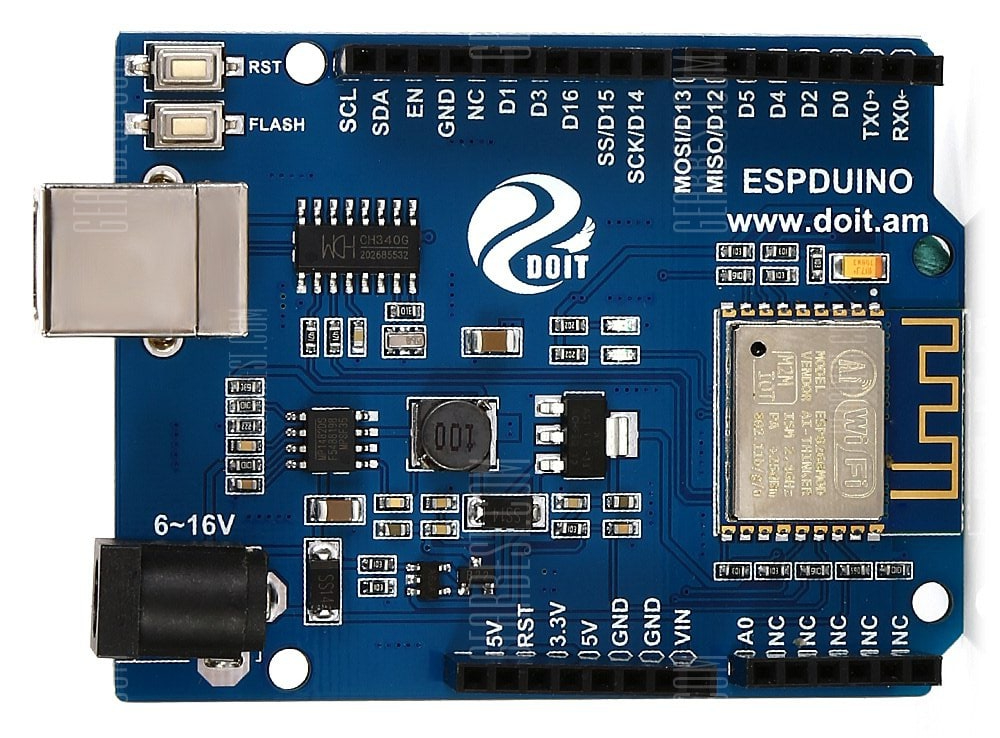
\includegraphics[keepaspectratio, width=0.4
\textwidth]{images/espduino.jpg}
\caption{ESPduino}
\label{fig:arduino}
\end{figure}

	Quando lançado no mercado, o ESP8266 não fez muito sucesso por não possuir documentação em inglês, porém, em outubro de 2014, a Espressif disponibilizou um kit de desenvolvimento de software (SDK) que permitiu que o chip fosse programado diretamente, sem a necessidade de um microcontrolador intermediário como vinha sendo feito até então. Desta forma, começaram a serem exploradas as potencialidades do ESP8266 e percebeu-se que sua capacidade era equivalente ou até mesmo superior a do microcontrolador Atmel presente nos Arduinos aos quais ele era utilizado como um simples módulo de wifi e, assim, surgiram projetos para a utilização do ESP8266 como um microcontrolador independente com os mesmos recursos dos Arduinos comuns.
    
    Dentre os projetos de uso do ESP8266, surgiu o ESPduino, que se baseia na estrutura da placa Arduino convencional, porém com o ESP8266 como microcontrolador ao invés do Atmel AVR, além do recurso de wifi já integrado a placa e a possibilidade de ser programado na linguagem de programação e IDE utilizados com o Arduino. Sendo assim, o ESPduino pode ser utilizado da mesma forma que um Arduíno convencional, possibilitando inclusive , a adição módulos de expansão de recursos.
    
	\section{Metodologia}
	O presente estudo trata-se da exploração de uma forma de ensino de programação em escolas que alia os conhecimentos ensinados em sala de aula com a aplicação prática em um ambiente real e acessível aos alunos, caracterizando assim uma pesquisa de cunho exploratório. No que tange a abordagem de pesquisa, este trabalho pode ser caracterizado como qualitativo, pois será analisada a eficiência, viabilidade e aceitação do método de ensino de programação proposto.
    
    Dado seu caráter de pesquisa aplicada, o trabalho contará com o apoio das escolas interessadas em contribuírem com o projeto, por meio da disponibilização do espaço físico e com os grupos de alunos motivados a participar das atividades.    
	
    \subsection{Análise das alternativas de ferramentas disponíveis}
    Nesta etapa serão pesquisadas as alternativas de ferramentas disponíveis e de fácil acesso e que sejam adequadas para a proposta. Serão elencadas as melhores opções encontradas, avaliando características como: disponibilidade, facilidade de uso, recursos disponíveis e qualidade.
    
    \subsection{Prototipação}
    Etapa na qual serão construídos protótipos funcionais do material de ensino proposto, no caso, os recursos de hardware e software necessários para o ensino de programação aplicado ao cenário da irrigação e monitoramento de uma horta escolar. 
    
    Como a proposta visa o funcionamento em um ambiente real, no contexto de uma horta, é de suma importância a consideração de fatores como a exposição as intempéries do clima, além da disponibilidade de recursos essenciais para o funcionamento do sistema como um todo. Desta forma, a fase de prototipagem torna-se indispensável para identificar possíveis deficiências e também melhorias do projeto antes de sua aplicação nas escolas.
    
    \subsection{Modularização}
    Como trata-se da proposta de um método de ensino de programação, é indispensável que se idealize uma metodologia de aplicação ao alunos que seja didática e que consiga cumprir sua proposta de transmitir o conteúdo. Pensando nisso, na etapa de modularização, todos os processos envolvidos na consolidação de um sistema de irrigação e monitoramento de uma horta escolar, voltada ao ensino de programação, serão classificados em espécies de "módulos de ensino", com o intuito de estabelecer uma ordem de progresso incremental na aprendizagem e de acordo com a complexidade de implementação. 
    
    Os módulos iniciais terão grau de dificuldade menor e os demais vão evoluindo sua complexidade até chegar nos módulos considerados de níveis mais avançados.
    
    \subsection{Execução do projeto em um cenário real}
   Por fim, a etapa de execução do projeto em um cenário real, será a implementação da abordagem de ensino de programação proposta em uma das possíveis escolas interessadas. Nesta fase, será ensinado aos alunos os preceitos de programação seguindo a metodologia estruturada pelo presente trabalho, fornecendo assim o feedback necessário para a validação da eficácia dessa proposta. 

	\section{Plano de Atividades e Cronograma}
	
	O cronograma de atividades será composto de 6 etapas. São elas:
    
    \begin{enumerate}
		\item \label{activity:pesquisa} \textbf{Pesquisa e análise das alternativas de ferramentas:} Atividade em que será realizado um levantamento das opções de ferramentas e materiais disponíveis visando definir quais tecnologias serão utilizadas durante o desenvolvimento do trabalho, algumas dessas tecnologias a serem buscadas e analisadas são: placas de prototipagem, sensores, serviços de armazenamento de dados online e materiais para confecção dos protótipos.
        
        \item \label{activity:prototipos} \textbf{Criação de protótipos funcionais:} Etapa na qual serão projetados e construídos os protótipos do sistema de irrigação e monitoramento de horta escolar, utilizando os materiais previamente elencados na seleção da etapa anterior. Além disso, os protótipos passarão por constantes testes para a identificação de problemas, possibilitando a correção prévia dos mesmos e a consequente melhoria dos protótipos.
        
        \item \label{activity:servidor} \textbf{Comunicação do sistema com um servidor:} Esta atividade consiste em analisar e implementar alguma alternativa para o armazenamento dos dados provenientes dos sensores que estarão dispostos na horta. Para possibilitar o acesso dos dados gerados fora da rede a qual o sistema está conectado, faz-se necessário o envio e armazenamento desses dados em um servidor online e externo a essa rede, portanto, é nessa etapa que serão estudadas e implantadas as melhores alternativas e serviços para dada finalidade.
        
        \item \label{activity:instalacao} \textbf{Instalação do sistema em uma escola:} Nesta etapa, será realizada a instalação do sistema de irrigação e monitoramento  na horta de, ao menos, uma das escolas interessadas.  
        
        \item \label{activity:alunos} \textbf{Montar uma turma de alunos para realização das atividades: } Sendo uma das principais atividades, a reunião de alunos para a aplicação das atividades do projeto, será realizada com alunos interessados no aprendizado de programação e estudantes das escolas colaboradoras. Tal etapa possui grande importância para o projeto, pois será a partir dela que se validará o trabalho desenvolvido.  
        
        \item \label{activity:feedback} \textbf{Obtenção e análise do feedback das atividades:} Serão analisados os feedbacks obtidos a partir da execução das atividades de aprendizado por parte dos alunos, além de identificar pontos importantes no processo como um todo, possibilitando ao fim, a obtenção de uma conclusão e discussão dos aspectos relevantes do trabalho. 
        
    \end{enumerate}
    
       \begin{table}[!ht]
		\centering
		\begin{tabular}{c|ccccc}
			Etapa & Agosto & Setembro & Outubro & Novembro & Dezembro \\ \hline
			\ref{activity:pesquisa} & \checkmark & & & & \\
			\ref{activity:prototipos} & \checkmark & \checkmark &  \\
			\ref{activity:servidor} & & \checkmark & \checkmark & \checkmark & \\
			\ref{activity:instalacao} & & \checkmark & \checkmark & \checkmark & \checkmark  \\
			\ref{activity:alunos} & & & \checkmark & \checkmark & \checkmark \\
            \ref{activity:feedback} & & & & \checkmark & \checkmark \\
		\end{tabular}
		\caption{Cronograma de Atividades}
	\end{table}
    
	\section{Recursos}
	 Como recursos físicos a serem utilizados neste projeto estão inclusos o computador pessoal do autor do trabalho, as placas de prototipação programáveis, ferramentas para a montagem dos protótipos, espaço físico da horta escolar, além das linguagens, API's e bibliotecas que auxiliarão tanto o autor quanto os alunos das escolas a quem se destina as atividades que serão propostas.
     
     Como colaboradores podem ser incluídos os alunos e professores das escolas interessadas no projeto, pois, mesmo não participando da idealização do trabalho, serão parte importante na fase de execução do mesmo.

	\section{Resultados Esperados}
Espera-se que a estratégia de ensino de programação proposta neste trabalho consiga cumprir o seu objetivo enquanto alternativa didática e possa ser vista como uma opção viável para se trabalhar com crianças e jovens. Além disso, também é esperado que, no decorrer da execução do trabalho nas escolas colaboradoras, seja despertado o interesse por parte dos alunos para o prosseguimento do projeto de irrigação e monitoramento da horta, instigando-se a identificação dos possíveis problemas e as melhorias a serem feitas.

	\bibliographystyle{abbrvnat}
	\bibliography{projeto} 
	
\end{document}
